\chapter{Mạng Internet với Raspberry Pi}
\section{Kết nối internet với dây mạng LAN}
Trên Raspberry Pi có hổ trợ cổng Ethernet, chúng ta có thể kết nối dây mạng trực tiếp vào đây.
\section{Kết nối internet với USB Wifi}
Trong phần này, mình sử dụng USB Wifi TP Link 725N
\subsection{Cài đặt Drive}
Tham khảo tại: \verb|https://www.raspberrypi.org/forums/viewtopic.php?p=462982|

Thực hiện theo các bước sau:
\begin{itemize}
\item Xác định phiên bản hệ điều hành Raspbain:
\begin{lstlisting}[language=make]
$ uname -a
Linux raspberrypi 4.1.13+ #826 PREEMPT Fri Nov 13 20:13:22 GMT 2015 armv6l GNU/Linux
\end{lstlisting}
Trong ví dụ trên, phiên bản hệ điều hành là \verb|4.1.13+ #826|. 
\item Vào địa chỉ bên dưới để tải drive:

\verb|https://www.raspberrypi.org/forums/viewtopic.php?p=462982|
\item Cài đặt drive, thực hiện các lệnh bên dưới:
\begin{lstlisting}[language=make]
wget https://dl.dropboxusercontent.com/u/80256631/8188eu-201xyyzz.tar.gz
tar -zxvf 8188eu-201xyyzz.tar.gz
sudo install -p -m 644 8188eu.ko /lib/modules/$(uname -r)/kernel/drivers/net/wireless
sudo insmod /lib/modules/$(uname -r)/kernel/drivers/net/wireless/8188eu.ko
sudo depmod -a
\end{lstlisting}
Đối với Raspberry Pi 2, chúng ta chỉ cần thực hiện 2 lệnh sau:
\begin{lstlisting}[language=make]
tar xzf 8188eu-2015yyzz.tar.gz
./install.sh
\end{lstlisting}
Với \verb|8188eu-201xyyzz.tar.gz| là drive phù hợp với phiên bản hệ điều hành của bạn.

Bạn có thể tải drive từ máy tính rồi chép vào Raspberry Pi để cài đặt (cách này dùng cho Pi chưa được kết nối với Internet).
\item[$\ast$] Trong quá trình cập nhật các phiên bản mới của hệ điều hành, khi đó Raspberry Pi không còn nhận USB Wifi nữa, lúc đó ta cần cài đặt Drive mới cho USB Wifi.
\end{itemize}
\subsection{Cài đặt địa chỉ IP tĩnh}
Tham khảo tại địa chỉ: 

\begin{footnotesize}
\verb|http://weworkweplay.com/play/automatically-connect-a-raspberry-pi-to-a-wifi-network/|
\end{footnotesize}\\

Ta sửa đổi nội dung của 2 tập tin dưới đây:
\begin{itemize}
\item Tập tin: \verb|interfaces|, mở tập tin:
\begin{lstlisting}[language=bash]
$ sudo nano /etc/network/interfaces
\end{lstlisting}
và thay đổi nội dung như sau:
\lstinputlisting[language=make]{interfaces}
\item Tập tin: \verb|wpa_supplicant.conf|,  mở tập tin:
\begin{lstlisting}[language=bash]
$ sudo nano /etc/wpa_supplicant/wpa_supplicant.conf
\end{lstlisting}
và thay đổi nội dung như sau:
\lstinputlisting[language=make]{wpa_supplicant.conf}
\end{itemize}
\section{Sử dụng chung Wifi với Laptop}
Ta kết nối cổng Ethernet của Pi và Laptop với nhau. Sử dụng tín năng Share Wifi trên Laptop:
\subsection{Hệ điều hành Ubuntu}
Thực hiện theo các bước sau:
\begin{itemize}
\item Trong thanh tìm kiếm \verb|Dash|: gõ vào \verb|Network Connections|, chọn \verb|Network Connections| để mở lên.
\begin{figure}[!h]
\begin{center}
{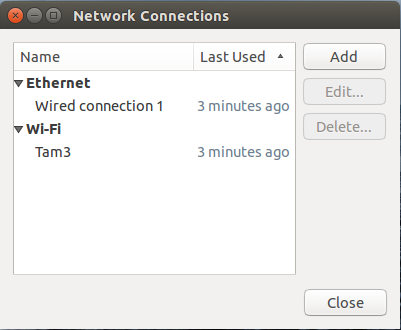
\includegraphics[scale=.5]{network/images/share-wifi-1}}
\end{center}
\caption{Mở \textsf{Network Connections}}
\end{figure}
\item Chọn \verb|Add|:
\begin{figure}[!h]
\begin{center}
{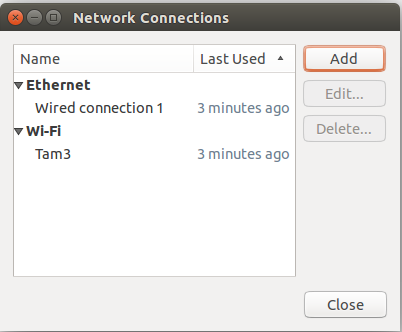
\includegraphics[scale=.5]{network/images/share-wifi-2}}
\end{center}
\caption{Chọn \textsf{Add}}
\end{figure}
\newpage
\item Chọn \verb|Create|:
\begin{figure}[!h]
\begin{center}
{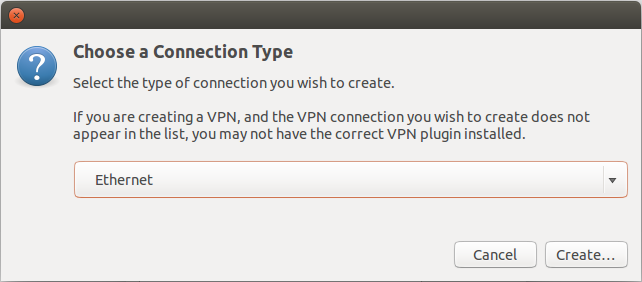
\includegraphics[scale=.4]{network/images/share-wifi-3}}
\end{center}
\caption{Chọn \textsf{Create\ldots}}
\end{figure}
\item Điền tên trong ô \verb|Connection name|:
\begin{figure}[!h]
\begin{center}
{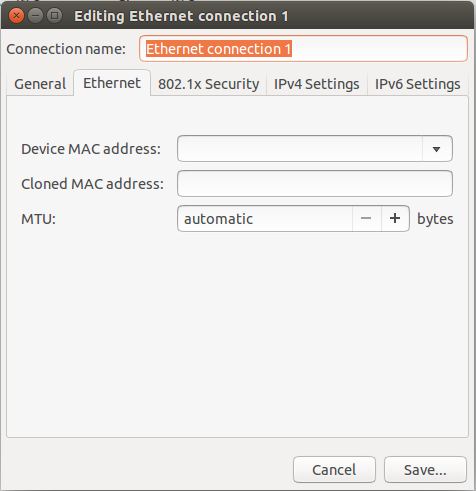
\includegraphics[scale=.4]{network/images/share-wifi-4}}
\caption{Điền tên trong ô \textsf{Connection name}}
\end{center}
\end{figure}
\item Chọn tab \verb|IPv6 Settings|, chọn \verb|Method| là \verb|Automactic|:
\begin{figure}[!h]
\begin{center}
{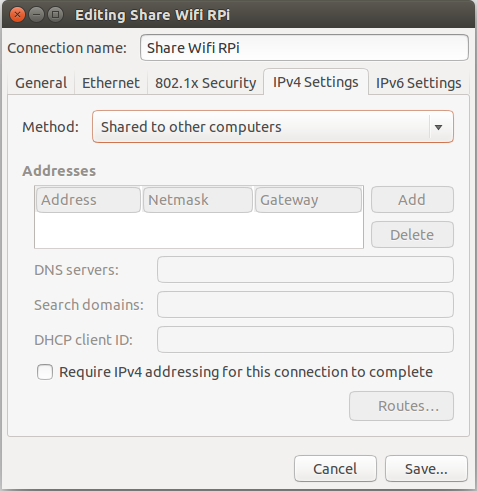
\includegraphics[scale=.4]{network/images/share-wifi-5}}
\caption{Chọn tab \textsf{IPv6 Settings}, chọn \textsf{Method} là \textsf{Automactic}}
\end{center}
\end{figure}
\item Chọn tab \verb|IPv4 Settings|, chọn \verb|Method| là \verb|Share to orther computers|:
\begin{figure}[!h]
\begin{center}
{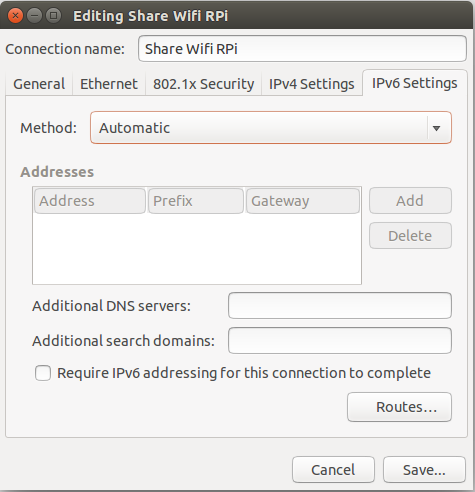
\includegraphics[scale=.5]{network/images/share-wifi-6}}
\caption{Chọn tab \textsf{IPv6 Settings}, chọn \textsf{Method} là \textsf{Share to orther computers}}
\end{center}
\end{figure}
\item Chọn \verb|Save| rồi chọn \verb|Close|.
\item Mở cửa sổ lệnh \verb|Terminal| gõ lệnh:
\begin{lstlisting}[language=bash]
$ sudo cat /var/lib/misc/dnsmasq.leases
1461927547 b8:27:eb:6a:bf:9a 10.42.0.31 raspberrypi ff:eb:6a:bf:9a:00:01:00:01:1c:dd:60:6b:b8:27:eb:6a:bf:9a
\end{lstlisting}
\item Địa chỉ của Pi lúc này là \verb|10.42.0.31|
\item Truy cập qua SSH bằng lệnh:
\begin{lstlisting}[language=bash]
$ ssh pi@10.42.0.31
\end{lstlisting}
\item Nhập password đăng nhập tài khoản username là \verb|pi|.
\end{itemize}